\section{Problem Analysis} % (fold)
\label{sec:analysis}

In this section we will analyze and describe our approach on implementing Raft with relation to the purpose of this project and with relation to achieve a more fault-tolerant and robust implementation.

\subsection{Existing Raft Implementations} % (fold)
\label{sub:existing_raft_implementations}

The application of consensus algorithms such as Raft is many, but the most generic applications are databases and service discovery systems. As Raft mostly fits applications in the low level end of the stack, it will also be best suited to be implemented in a more low level and light language such as C, C++ or Go. Erlang would also be a great fit with its fault-tolerant features.

Raft have already been implemented in several versions and in many languages. Diego Ongaro himself has implemented Raft in C++ (LogCabin\footnote{https://github.com/logcabin/logcabin}), CoreOS\footnote{A new Linux operation system fork made for server deployments.} uses etcd\footnote{https://github.com/coreos/etcd}, which is a Raft implementation in Go used for service discovery.

If a Raft implementation was needed for real usage, the solution would have been to extend some of the rich open source implementations already available in solid languages as Go and C. But as mentioned in the introduction, the scope of this project is to learn about Raft with relation to fault-tolerance by implementing it. To be able to cover as much of Raft as possible in the time scope, the language chosen for implementation is JavaScript, because it would allow more productivity.

There already exists solutions in JavaSciript, but since one of the focus of this project is to learn about Raft and the consensus problem, we have chosen to implement a new version with our own approach. Already existsing solutions in JavaScript such as \href{https://github.com/ongardie/raftscope}{raftscope} and \href{https://github.com/pgte/skiff-algorithm}{skiff} have worked as inspirations during implementation.

% subsection existing_raft_implementations (end)

\subsection{Testing} % (fold)
\label{sub:testing}

In order to be able to verify that the implementation satisfies the requirements and that to ensure a higher level of robustness, the software will be thoroughly tested. To document requirement satisfaction, the implementation will be black-box tested on the level of acceptance and integration.

In order to achieve robustness the implementation will also be white-box tested on the unit test level in order to test the behaviour of the different objects in situations and cases that are hard to foresee.

% subsection testing (end)

\subsection{Development Approach}
\label{sub:development_approach}

The Raft paper includes an informal specification~\cite[page~4]{Raft} with behaviour of the servers described by the state they are in or how to respond to requests. In order to have a more common language between the specification and the tests, the development approach Behaviour Driven Development (BDD) was chosen\footnote{Originally described by Dan North in the blog post \url{http://dannorth.net/introducing-bdd/}}~\cite{bddpaper}. The Behaviour Driven approach is iterative and have been used in the report with the following steps:

\begin{enumerate}
    \item Derive behaviour from the specification and write a failing test of the given behaviour.
    \item Write the simplest code that implements the behaviour and make the test pass.
    \item Refactor the code
    \item Repeat
\end{enumerate}

This is close to Test Driven Development, but with focus on writing tests that describes behaviour instead of testing methods as in unit tests.
One important aspect to make this approach work well is to derive the behaviour that seem most easy to implement first.

To facilitate writing tests with a BDD-aproach, we used the node lirbaries \href{http://chaijs.com/}{\tt chai} together with \href{http://mochajs.org}{\tt mocha}, which allows us to write tests written as behaviour such as the example seen in code examplre below.

\lstinputlisting[caption=Example of a JavaScript test with the libraries mocha and chai, language=JavaScript]{code_snippets/chai_mocha_example.js}

% subsection our_approach (end)

\subsection{Visualization Tool} % (fold)
\label{sub:visualization_tool}

An extended requirement specified in section~\ref{sec:requirements} was to build a visualization of the simulation tool. To be able to use the Raft implementation such that the visualization tool does not affect other extensions it is important to build it independent from each other as seen on figure~\ref{fig:algorithm_extension_visualization}. As visualization platform we have chosen to use the command line to visualize the simulation since it is the simplest one.

\begin{figure}[h]
  \centering
  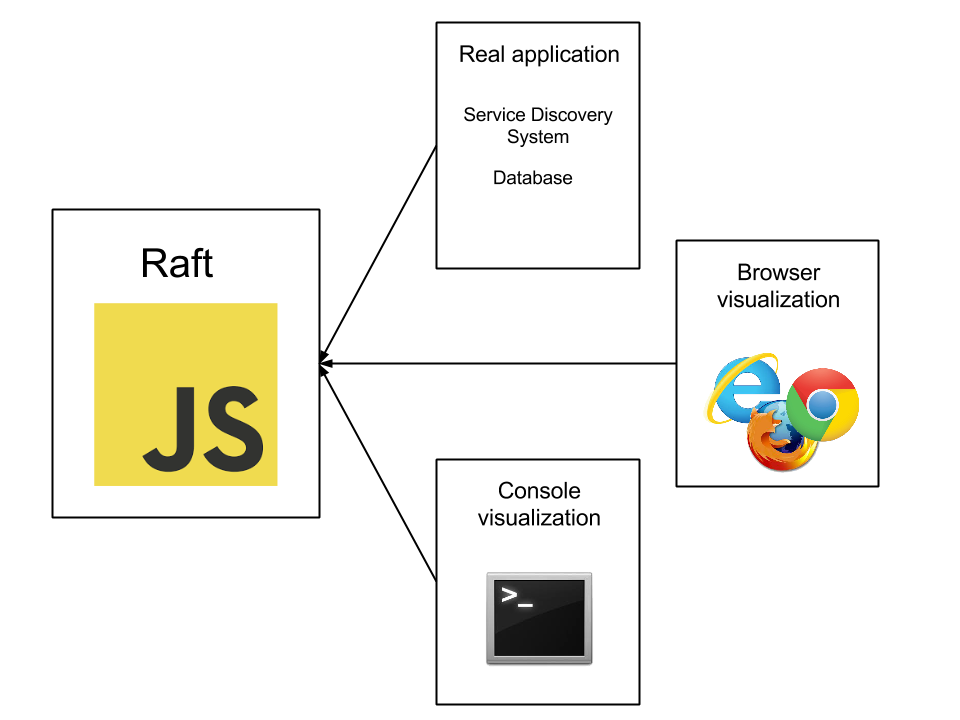
\includegraphics[width=0.5\textwidth]{figures/implementation_extensions.png}
  \caption{Illustrating how Raft should be implemented such that it is extendable for uses such as command line tools, browser visualizations or a real usage such as databases or service discovery systems.}
  \label{fig:algorithm_extension_visualization}
\end{figure}

% subsection visualization_tool (end)

% section analysis (end)
